\input{../header_1_en.tex}




\usepackage{Sweave}
\begin{document}

\begin{frame}[allowframebreaks]
  \titlepage
\end{frame}

\section*{Class outline}

\begin{frame}[allowframebreaks]
  \frametitle{Advanced Plotting}
  \tableofcontents[hideallsubsections]
\end{frame}

%%%%%%%%%%%%%%%%%%%%%%%%%%%%%%%%%%%%%%%%%%%%%%%%%%%%%%%%%%%%%%%%%%%%%%%%%%%
\section{intro}

\begin{frame}[allowframebreaks]
  \frametitle{\pl{R} is strong in plots}
  \begin{itemize}
  \item As you might recall, \pl{R} is very strong for making \BIOCfunction{plots}, and it does so fast.
  \item We've seen how to make barplots, qqplots, mosaicplots, and many other ones.
  \item After all, plotting is very important for doing \alert{exploratory data analysis}.
  \item However, all of them just make a small part.
  \end{itemize}
\end{frame}

\begin{frame}[allowframebreaks, fragile]
  \frametitle{Install some packages}
  To gain some time, please install these packages:
\begin{Schunk}
\begin{Sinput}
> install.packages("lattice")
> install.packages("mlmRev")
> install.packages("plotrix")
> install.packages("ggplot2")
> install.packages("car")
> install.packages("DAAG")
\end{Sinput}
\end{Schunk}
\end{frame}

\begin{frame}[allowframebreaks]
  \frametitle{Task Views}
  \begin{itemize}
  \item First of all, remember the CRAN \alert{Task Views}.
  \item \url{http://cran.r-project.org/web/views/Graphics.html}
  \item From there, go to the \pl{plotrix} page.
  \item What two functions did they introduce on version 2.5-3?
  \end{itemize}
\end{frame}

\begin{frame}[allowframebreaks, fragile]
  \frametitle{tools}
  \begin{itemize}
  \item You might decide to check the reference manual and test out the examples, but that's quite time consuming.
  \item I found out on the \BIOCfunction{R Journal} about a new function on the \pl{tools} package.
\begin{Schunk}
\begin{Sinput}
> library(tools)
> testInstalledPackage(pkgname)
\end{Sinput}
\end{Schunk}
  \item Its very \alert{easy} to create pdf files with all the example plots of a given package!
  \end{itemize}
\end{frame}

\begin{frame}[allowframebreaks, fragile]
  \frametitle{Remember to check the help}
  \begin{itemize}
  \item Remember to use:
\begin{Schunk}
\begin{Sinput}
> help.start()
> help(package = pkgname)
\end{Sinput}
\end{Schunk}
  \item What is the replacement of the \BIOCfunction{hist} function on the lattice package?
  \end{itemize}
\end{frame}

%%%%%%%%%%%%%%%%%%%%%%%%%%%%%%%%%%%%%%%%%%%%%%%%%%%%%%%%%%%%%%%%%%%%%%%%%%%
\section{lattice}

\begin{frame}[allowframebreaks, fragile]
  \frametitle{Intro}
  \begin{itemize}
  \item It's an \emph{implementation} of Trellis graphics and created by \BIOCfunction{Deepayan Sarkar}.
  \item \url{http://dsarkar.fhcrc.org/}
  \item Basically, its great for plotting multivariate data!
\begin{Schunk}
\begin{Sinput}
> `?`(Lattice)
\end{Sinput}
\end{Schunk}
  \item How are the lattice high level functions \alert{special}?
  \end{itemize}
\end{frame}

\begin{frame}[allowframebreaks, fragile]
  \frametitle{Data}
  \begin{itemize}
  \item We'll use a data set from the \pl{mlmRev} package and in general we'll follow the BioC2008 lattice lab.
\begin{Schunk}
\begin{Sinput}
> library(lattice)
> data(Chem97, package = "mlmRev")
\end{Sinput}
\end{Schunk}
  \item What is the class of \BIOCfunction{Chem97}?
  \item How many variables does it have? \emph{You might want to use length}
  \end{itemize}
\end{frame}

\begin{frame}[allowframebreaks]
  \frametitle{Formula syntax}
  \begin{itemize}
  \item We'll mostly use three variables: score, gcsescore and gender. 
  \item Now, \BIOCfunction{lattice} uses the \alert{formula} syntax.
  \item Basically its $y ~ x | g1$ where $x$ is the variable with the numeric values and $g1$ is a factor.
  \end{itemize}
\end{frame}

\begin{frame}[fragile, allowframebreaks]
  \frametitle{Comparing histograms}
\begin{Schunk}
\begin{Sinput}
> hist(Chem97$gcsescore)
\end{Sinput}
\end{Schunk}
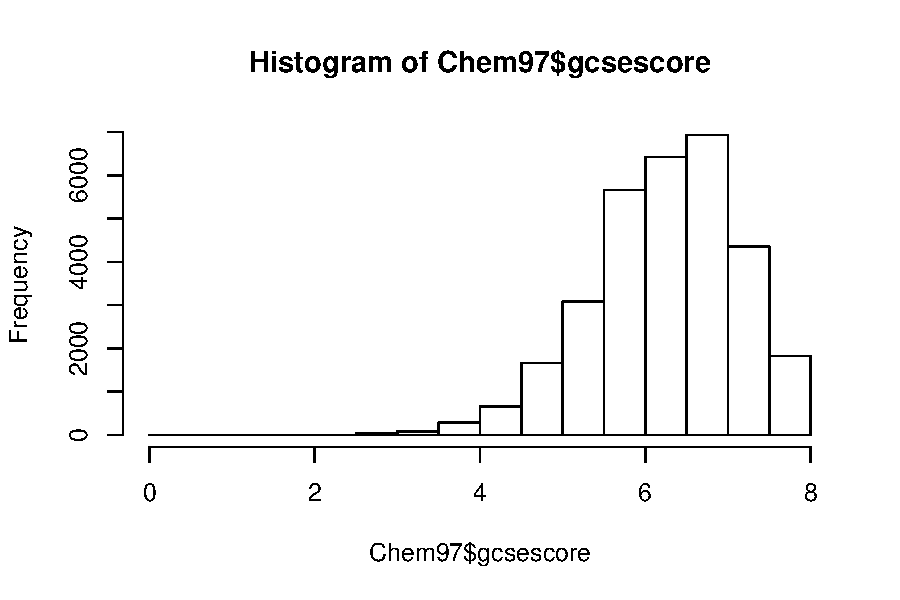
\includegraphics{plots/fig-007}
\end{frame}

\begin{frame}[fragile, allowframebreaks]
  \frametitle{Comparing histograms: part II}
\begin{Schunk}
\begin{Sinput}
> print(histogram(~gcsescore, data = Chem97))
\end{Sinput}
\end{Schunk}
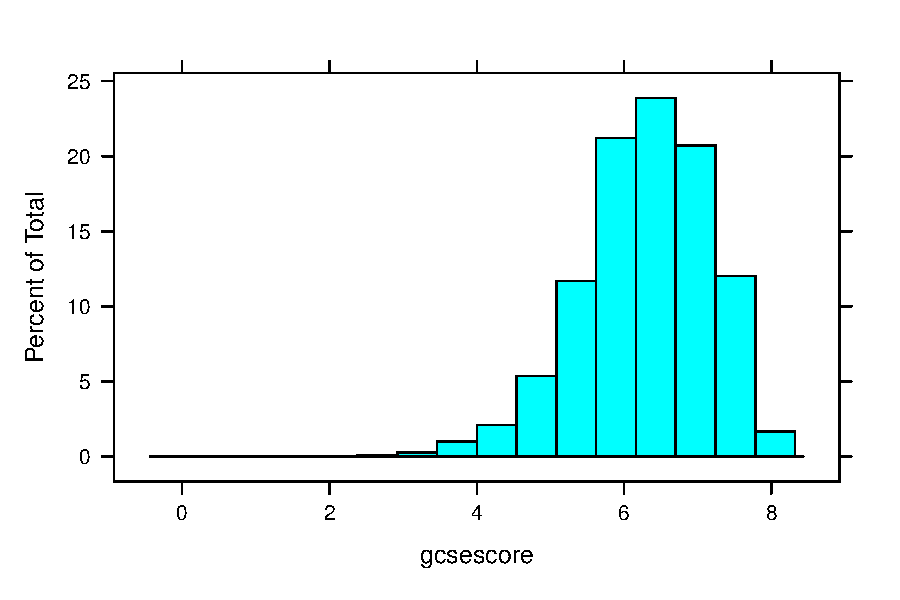
\includegraphics{plots/fig-008}
\end{frame}

\begin{frame}[allowframebreaks, fragile]
  \frametitle{A grouping var}
  \begin{itemize}
  \item The variable \pl{score} \alert{only} has values 0, 2, 4, 6, 8 and 10.
\begin{Schunk}
\begin{Sinput}
> head(Chem97$score)
\end{Sinput}
\begin{Soutput}
[1]  4 10 10 10  8 10
\end{Soutput}
\begin{Sinput}
> class(Chem97$score)
\end{Sinput}
\begin{Soutput}
[1] "numeric"
\end{Soutput}
\end{Schunk}
  \item We can use this variable as a factor!
  \item Lets make a more interesting plot :)
  \end{itemize}
\end{frame}

\begin{frame}[fragile, allowframebreaks]
  \frametitle{Multiple hist}
\begin{Schunk}
\begin{Sinput}
> print(histogram(~gcsescore | factor(score), 
+     data = Chem97))
\end{Sinput}
\end{Schunk}
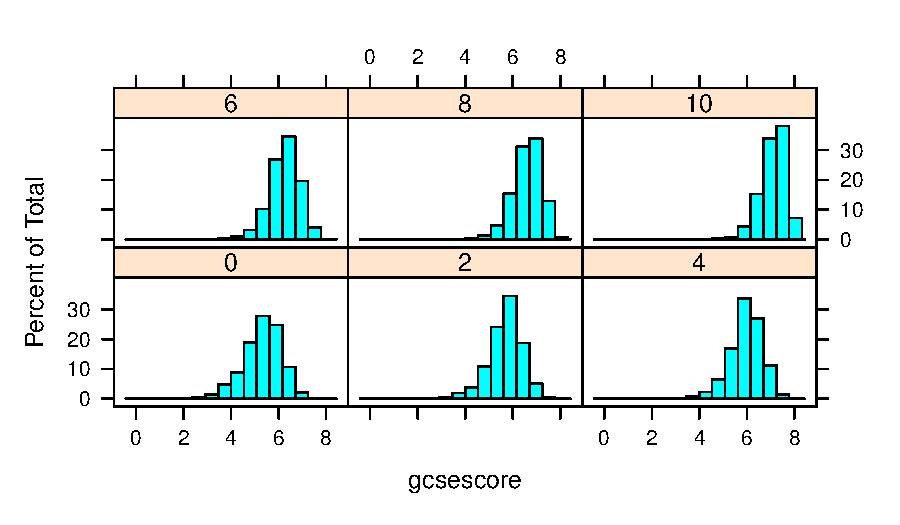
\includegraphics{plots/fig-010}
\end{frame}

\begin{frame}[allowframebreaks, fragile]
  \frametitle{And gender?}
  \begin{itemize}
  \item But we want to use our third variable: gender
\begin{Schunk}
\begin{Sinput}
> class(Chem97$gender)
\end{Sinput}
\begin{Soutput}
[1] "factor"
\end{Soutput}
\end{Schunk}
  \item Its \alert{difficult} to plot two histograms on the same panel, but that's not the case with density lines!
  \end{itemize}
\end{frame}

\begin{frame}[fragile, allowframebreaks]
  \frametitle{Densities}
\begin{Schunk}
\begin{Sinput}
> print(densityplot(~gcsescore | 
+     factor(score), Chem97, groups = gender, 
+     plot.points = FALSE, auto.key = TRUE))
\end{Sinput}
\end{Schunk}
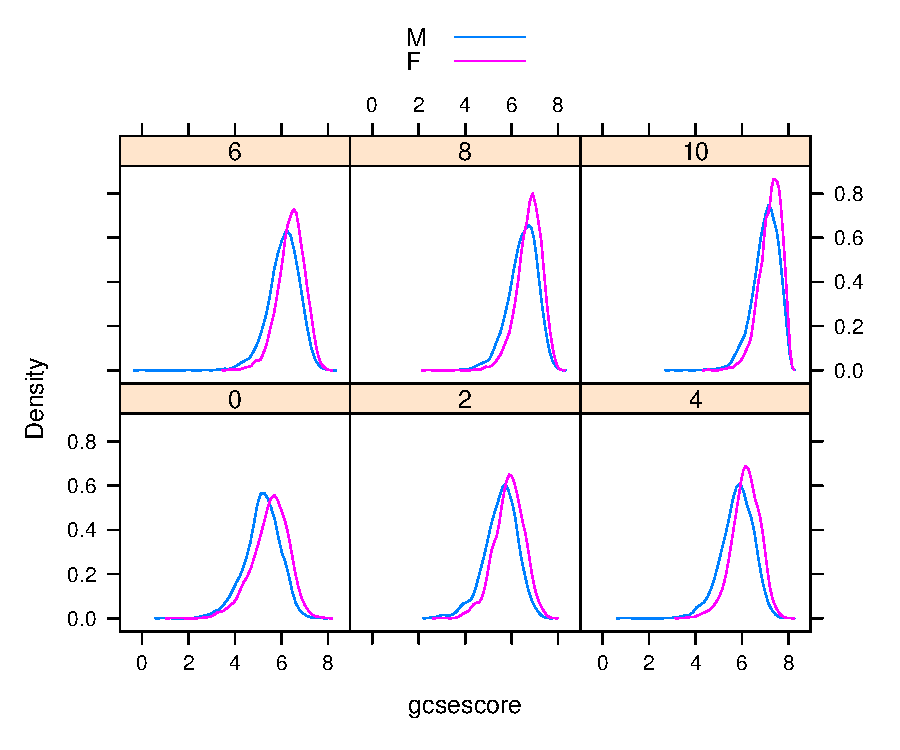
\includegraphics{plots/fig-012}
\end{frame}

\begin{frame}[fragile, allowframebreaks]
  \frametitle{QQ norm too!}
\begin{Schunk}
\begin{Sinput}
> print(qqmath(~gcsescore | factor(score), 
+     Chem97, groups = gender, auto.key = TRUE, 
+     aspect = "xy", f.value = ppoints(1000)))
\end{Sinput}
\end{Schunk}
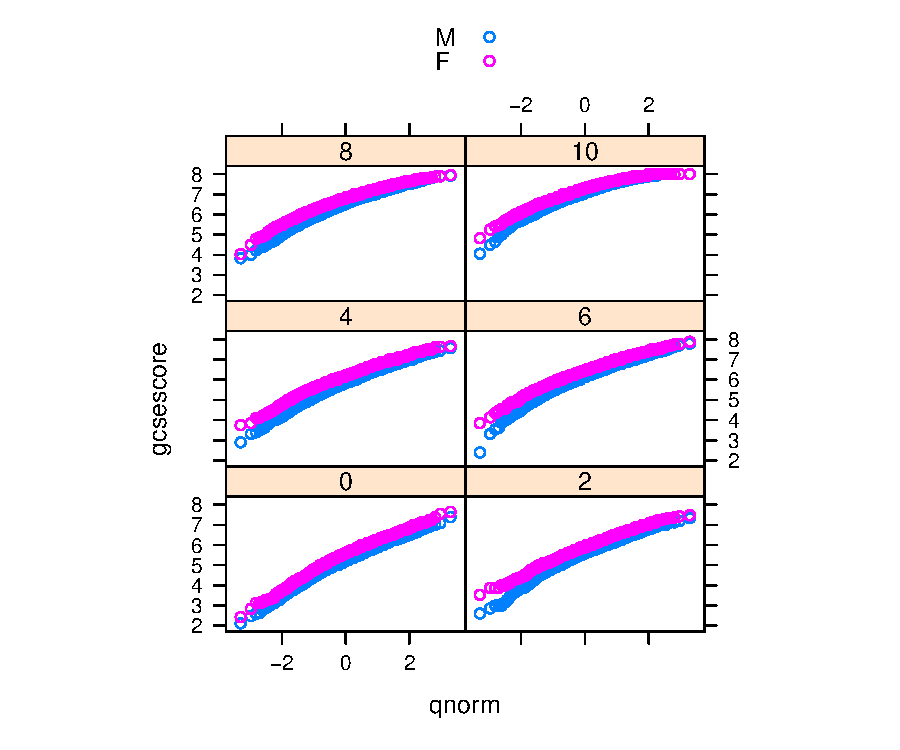
\includegraphics{plots/fig-013}
\end{frame}

\begin{frame}[allowframebreaks, fragile]
  \frametitle{Compare QQ norm}
  \begin{itemize}
  \item Re-do the above QQ norm plot with the following arguments:
\begin{Schunk}
\begin{Sinput}
> f.value = ppoints(100)
> type = c("p", "g")
\end{Sinput}
\end{Schunk}
  \item Which of the two QQ norm plots is clearer?
  \end{itemize}
\end{frame}

\begin{frame}[fragile, allowframebreaks]
  \frametitle{QQ plots}
\begin{Schunk}
\begin{Sinput}
> print(qq(gender ~ gcsescore | factor(score), 
+     Chem97, f.value = ppoints(100), 
+     type = c("p", "g"), aspect = 1))
\end{Sinput}
\end{Schunk}
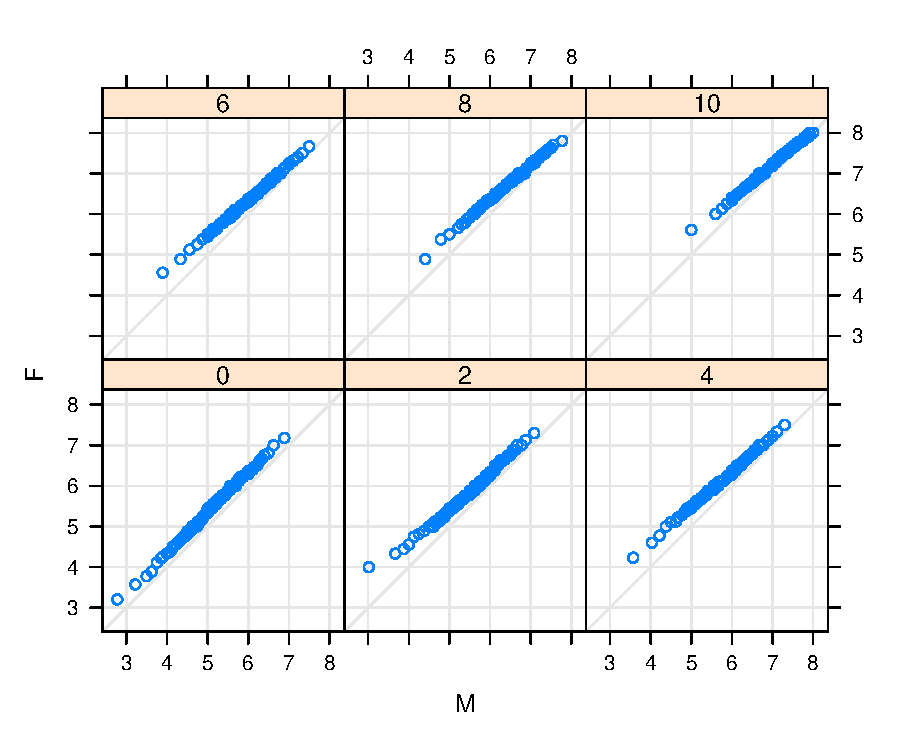
\includegraphics{plots/fig-015}
\end{frame}

\begin{frame}[fragile, allowframebreaks]
  \frametitle{Boxplots}
\begin{Schunk}
\begin{Sinput}
> print(bwplot(factor(score) ~ gcsescore | 
+     gender, Chem97))
\end{Sinput}
\end{Schunk}
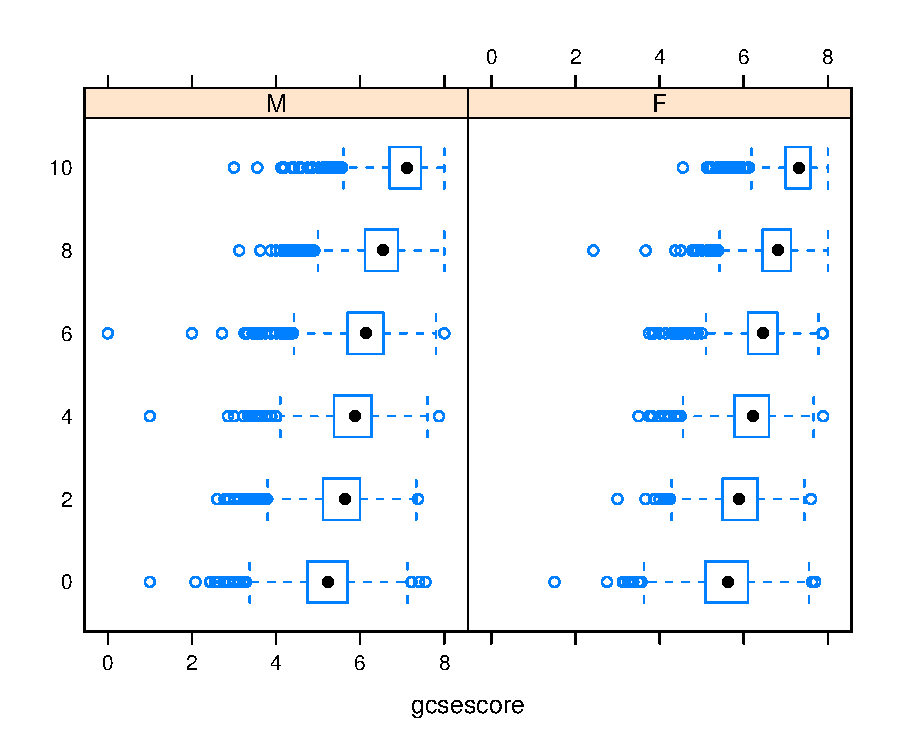
\includegraphics{plots/fig-016}
\end{frame}

\begin{frame}[fragile, allowframebreaks]
  \frametitle{Boxplots II}
\begin{Schunk}
\begin{Sinput}
> print(bwplot(gcsescore ~ gender | 
+     factor(score), Chem97, layout = c(6, 
+     1)))
\end{Sinput}
\end{Schunk}
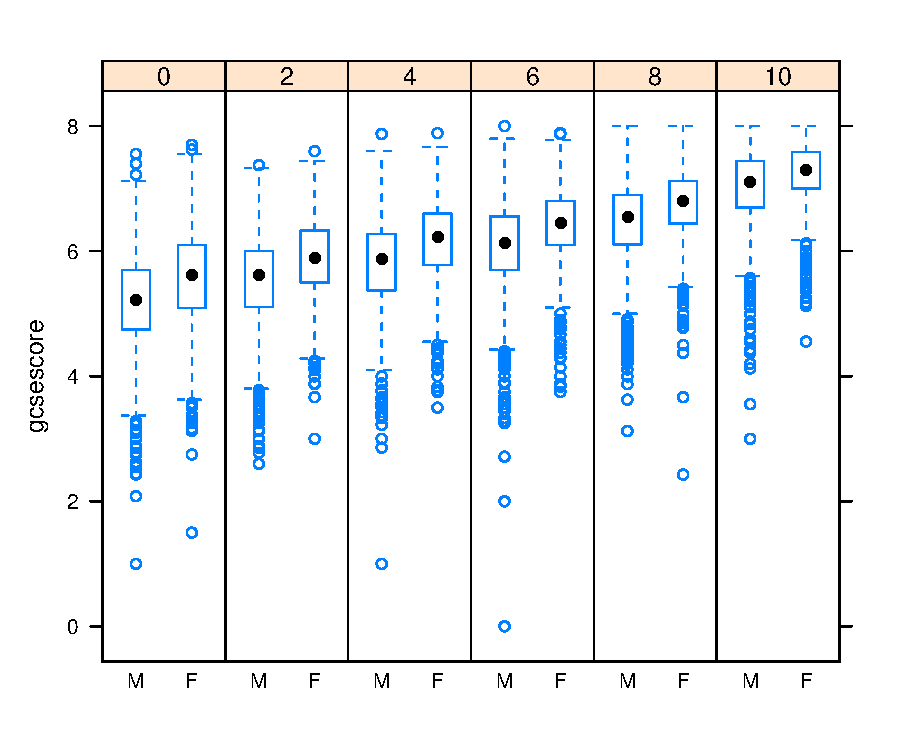
\includegraphics{plots/fig-017}
\end{frame}

\begin{frame}[fragile, allowframebreaks]
  \frametitle{Stripplot}
  \begin{itemize}
  \item Useful for small data sets :)
  \end{itemize}
\begin{Schunk}
\begin{Sinput}
> library(DAAG)
> print(stripplot(ht ~ factor(sport), 
+     data = ais))
\end{Sinput}
\end{Schunk}
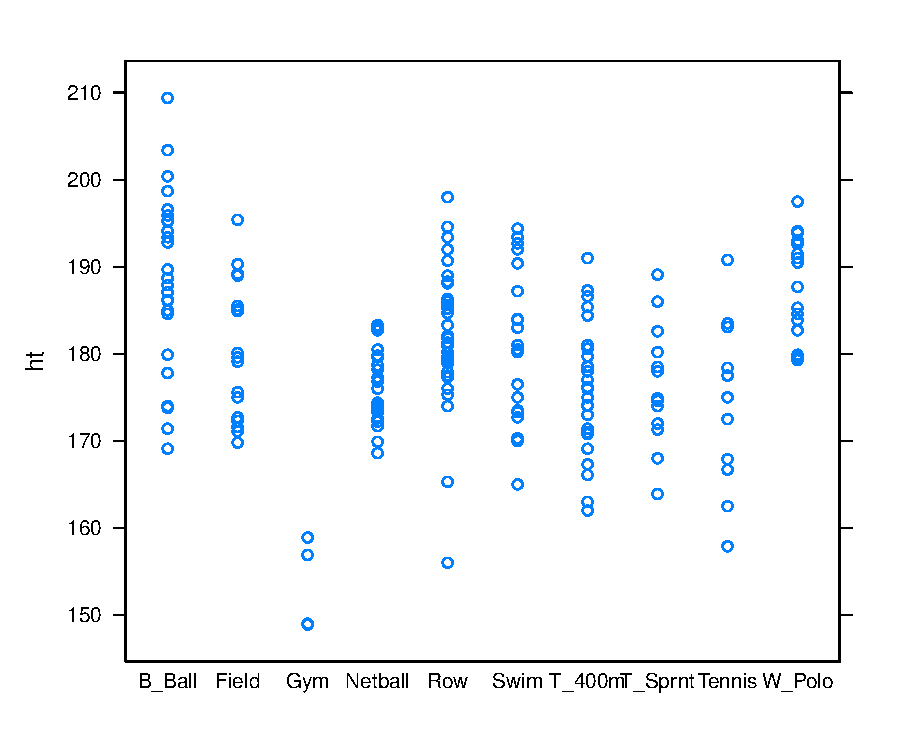
\includegraphics{plots/fig-018}
\end{frame}

\begin{frame}[fragile, allowframebreaks]
  \frametitle{Stripplot II}
  \begin{itemize}
  \item The \BIOCfunction{jitter} argument saves the day!
  \item Plus points in lattice are partially transparent
  \end{itemize}
\begin{Schunk}
\begin{Sinput}
> print(stripplot(ht ~ factor(sport), 
+     data = ais, jitter = T))
\end{Sinput}
\end{Schunk}
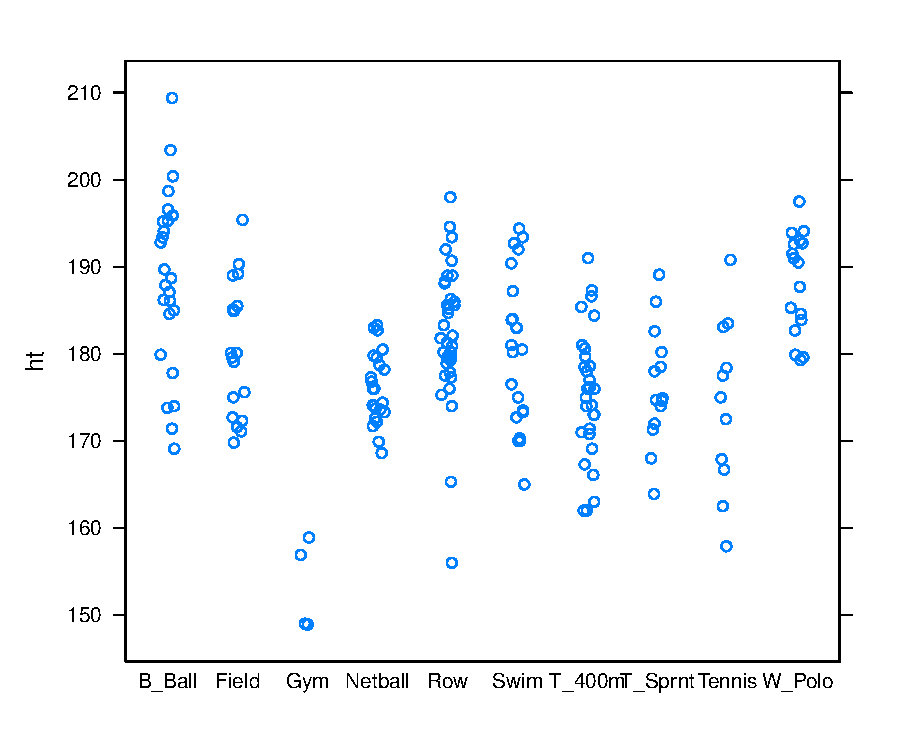
\includegraphics{plots/fig-019}
\end{frame}

\begin{frame}[fragile, allowframebreaks]
  \frametitle{xyplot}
  \begin{itemize}
  \item With lattice, we can also make something similar to \BIOCfunction{plot}
  \item But first, lets create a subset of the type of sports.
  \end{itemize}
\begin{Schunk}
\begin{Sinput}
> subset <- ais$sport %in% c("Netball", 
+     "Tennis")
> print(xyplot(ht ~ wt | sport, groups = sex, 
+     pch = c(4, 1), aspect = 1, 
+     subset = subset, data = ais))
\end{Sinput}
\end{Schunk}
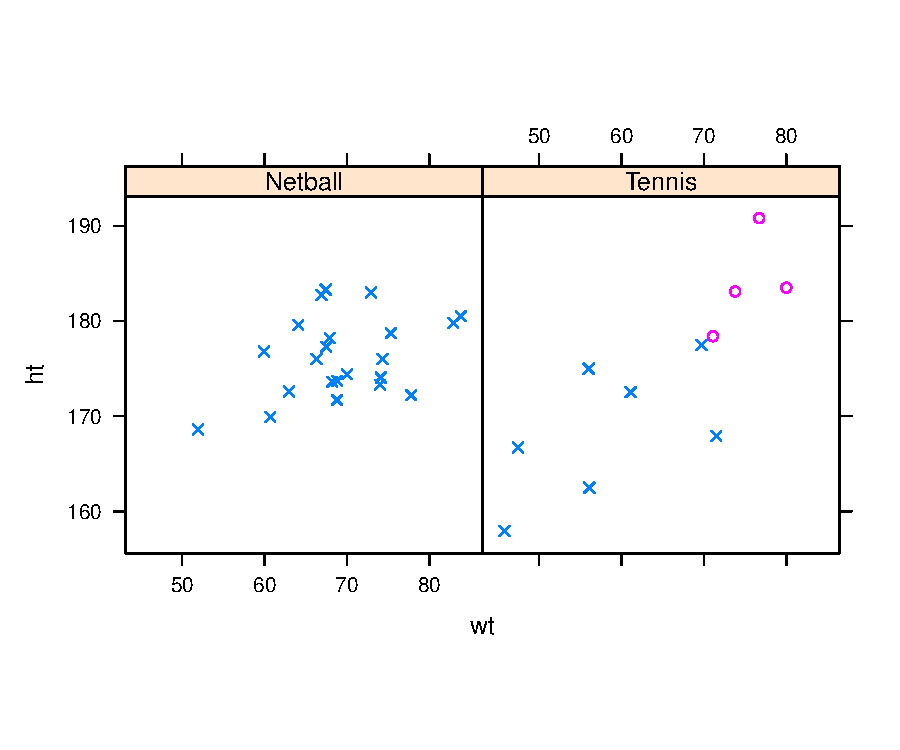
\includegraphics{plots/fig-020}
\end{frame}

\begin{frame}[fragile, allowframebreaks]
  \frametitle{xyplot II}
  \begin{itemize}
  \item What will happen if we say \pl{auto.key=TRUE}?
  \item On this plot, we are visualizing data from how many variables?
  \end{itemize}
\begin{Schunk}
\begin{Sinput}
> print(xyplot(ht ~ wt | sport, groups = sex, 
+     pch = c(4, 1), aspect = 1, 
+     auto.key = list(columns = 2), 
+     subset = subset, data = ais))
\end{Sinput}
\end{Schunk}
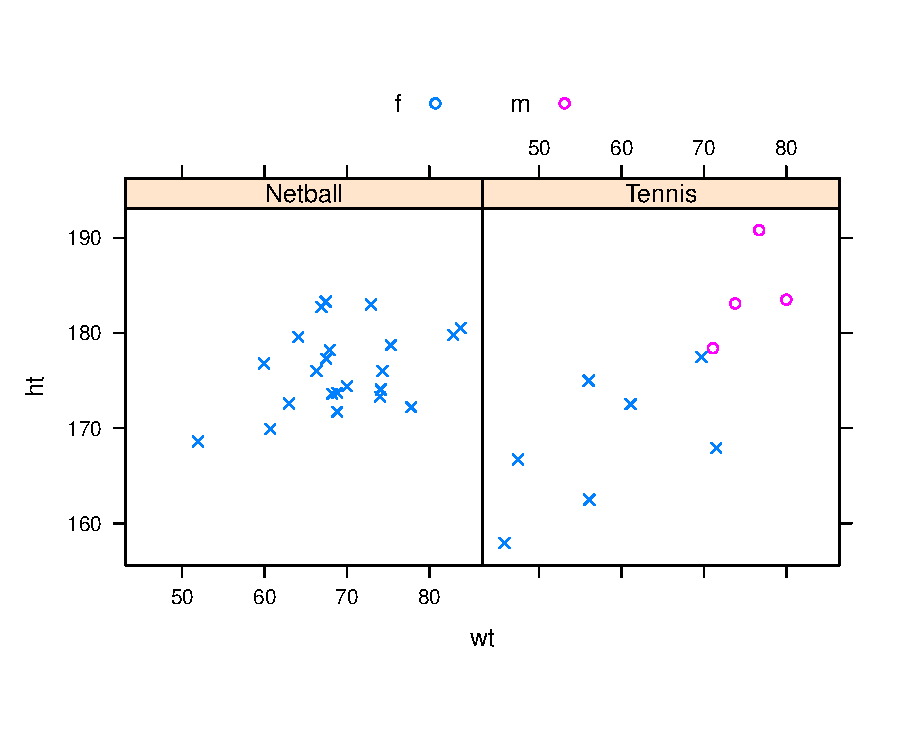
\includegraphics{plots/fig-021}
\end{frame}

\begin{frame}[fragile, allowframebreaks]
  \frametitle{xyplot B}
\begin{Schunk}
\begin{Sinput}
> data(Earthquake, package = "nlme")
> print(xyplot(accel ~ distance, 
+     data = Earthquake))
\end{Sinput}
\end{Schunk}
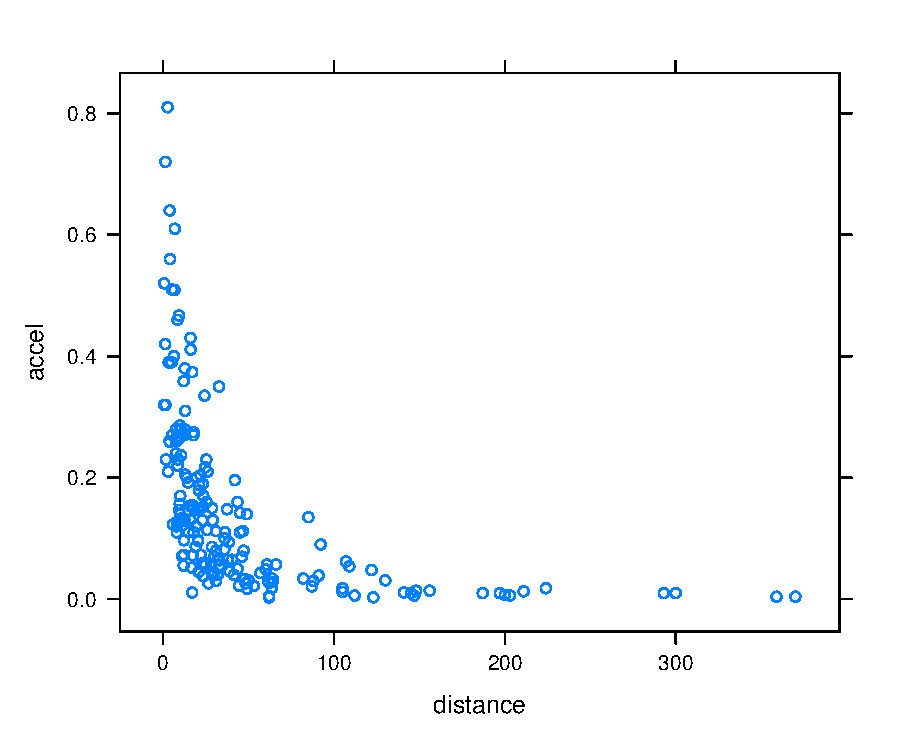
\includegraphics{plots/fig-022}
\end{frame}

\begin{frame}[fragile, allowframebreaks]
  \frametitle{xyplot B II}
  \begin{itemize}
  \item What does the \pl{scales} argument control?
  \item What would happen if you delete \pl{smooth} from the type argument?
  \end{itemize}
\begin{Schunk}
\begin{Sinput}
> print(xyplot(accel ~ distance, 
+     data = Earthquake, scales = list(log = TRUE), 
+     type = c("p", "g", "smooth"), 
+     xlab = "Distance From Epicenter (km)", 
+     ylab = "Maximum Horizontal Acceleration (g)"))
\end{Sinput}
\end{Schunk}
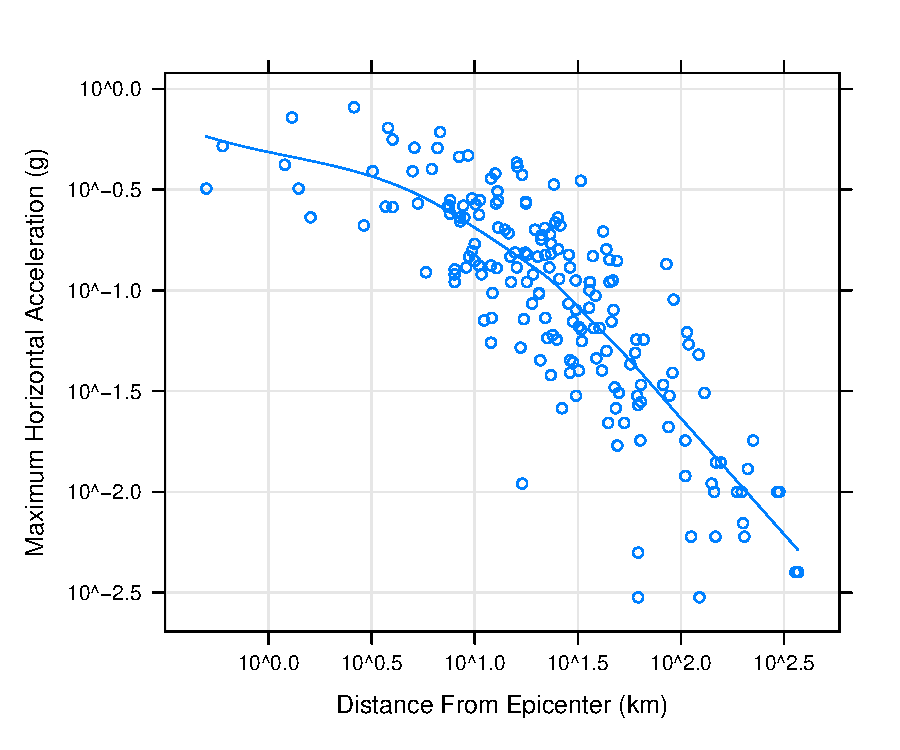
\includegraphics{plots/fig-023}
\end{frame}

\begin{frame}[fragile, allowframebreaks]
  \frametitle{3D!}
  \begin{itemize}
  \item With the \BIOCfunction{cloud} function its possible to create 3D plots. 
  \item To rotate it, you need to re-make it with different values for the $x$, $y$ and $z$.
  \end{itemize}
\begin{Schunk}
\begin{Sinput}
> print(cloud(depth ~ lat * long, 
+     data = quakes, zlim = rev(range(quakes$depth)), 
+     screen = list(z = 115, x = -60), 
+     panel.aspect = 0.75, xlab = "Longitude", 
+     ylab = "Latitude", zlab = "Depth"))
\end{Sinput}
\end{Schunk}
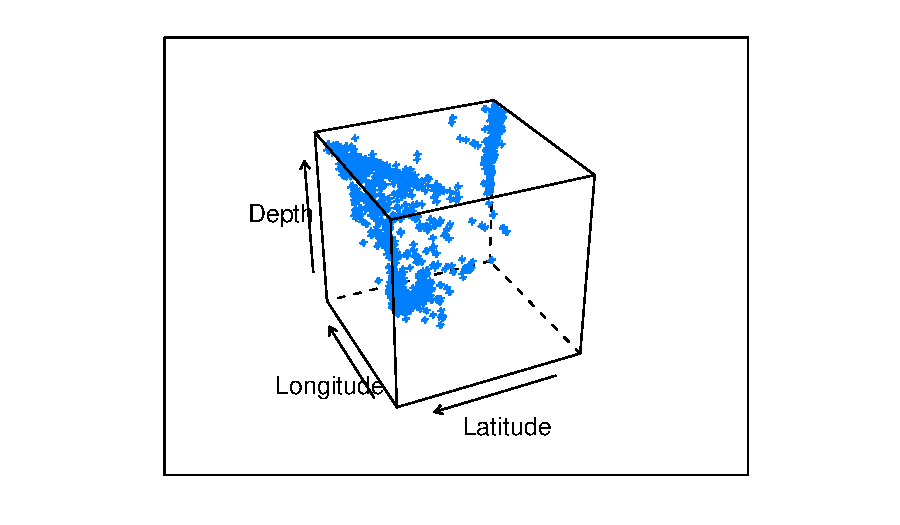
\includegraphics{plots/fig-024}
\end{frame}

\begin{frame}[allowframebreaks]
  \frametitle{That's it for lattice}
  \begin{itemize}
  \item \BIOCfunction{Lattice} has more plot functions such as \BIOCfunction{barchart} and \BIOCfunction{dotplot} which we won't cover today, but feel free to check them.
  \item There is also a book available on \pl{lattice}: \url{http://lmdvr.r-forge.r-project.org/}
  \item As I said at the beginning, use the \alert{\pl{tools}} package to explore \pl{lattice} and \pl{latticeExtra}.
  \end{itemize}
\end{frame}

%%%%%%%%%%%%%%%%%%%%%%%%%%%%%%%%%%%%%%%%%%%%%%%%%%%%%%%%%%%%%%%%%%%%%%%%%%%
\section{plotrix}

\begin{frame}[allowframebreaks]
  \frametitle{Intro}
  \begin{itemize}
  \item It contains loads of enhanced \pl{R} functions.
  \item The reference manual has \alert{139} pages!!!
  \item Functions such as adding a table, standard deviation bars, cutting axes, etc.
  \end{itemize}
\end{frame}

\begin{frame}[fragile, allowframebreaks]
  \frametitle{Barplot with table}
  \begin{itemize}
  \item First, we'll create a data.frame with some data
  \item Then we'll use the \BIOCfunction{barp} function to create a barplot
  \item Finally, we'll add the table to our plot
  \end{itemize}
\begin{Schunk}
\begin{Sinput}
> set.seed(123)
> df <- data.frame(Time0 = runif(3), 
+     Time1 = rnorm(3), Time2 = rlnorm(3))
> df <- round(df, digits = 2)
> rownames(df) <- c("Gene1", "Gene2", 
+     "Gene3")
> df
\end{Sinput}
\begin{Soutput}
      Time0 Time1 Time2
Gene1  0.29  1.19  0.90
Gene2  0.79 -1.69  0.89
Gene3  0.41  1.24  1.20
\end{Soutput}
\begin{Sinput}
> library(plotrix)
> barp(df, ylab = "Expression Lvl vs Control", 
+     names.arg = colnames(df), col = 1:3)
> addtable2plot(0.45, -1, df, bty = "o", 
+     display.rownames = TRUE, hlines = TRUE, 
+     title = "Data in table format")
\end{Sinput}
\end{Schunk}
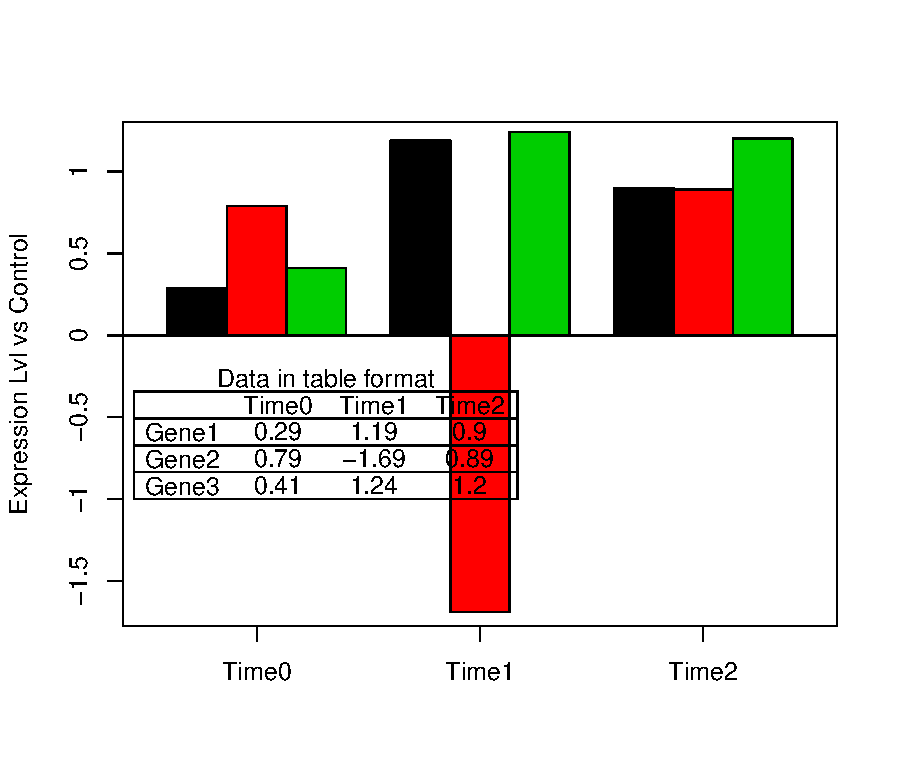
\includegraphics{plots/fig-025}
\end{frame}

\begin{frame}[fragile, allowframebreaks]
  \frametitle{Plot with gaps}
  \begin{itemize}
  \item With Plotrix we can make plots that have a gap on one axis.
  \item For example, a normal \pl{plot} with a gap on the $Y$ axis.
  \end{itemize}
\begin{Schunk}
\begin{Sinput}
> data <- c(rnorm(8) + 3, rnorm(8) + 
+     21, rnorm(8) + 4.5, rnorm(8) + 
+     20)
> color <- c(rep(2, 8), rep(3, 8), 
+     rep(4, 8), rep(1, 8))
> gap.plot(data, gap = c(8, 16), 
+     xlab = "Index", ylab = "Values", 
+     main = "Gap on Y axis", col = color)
\end{Sinput}
\end{Schunk}
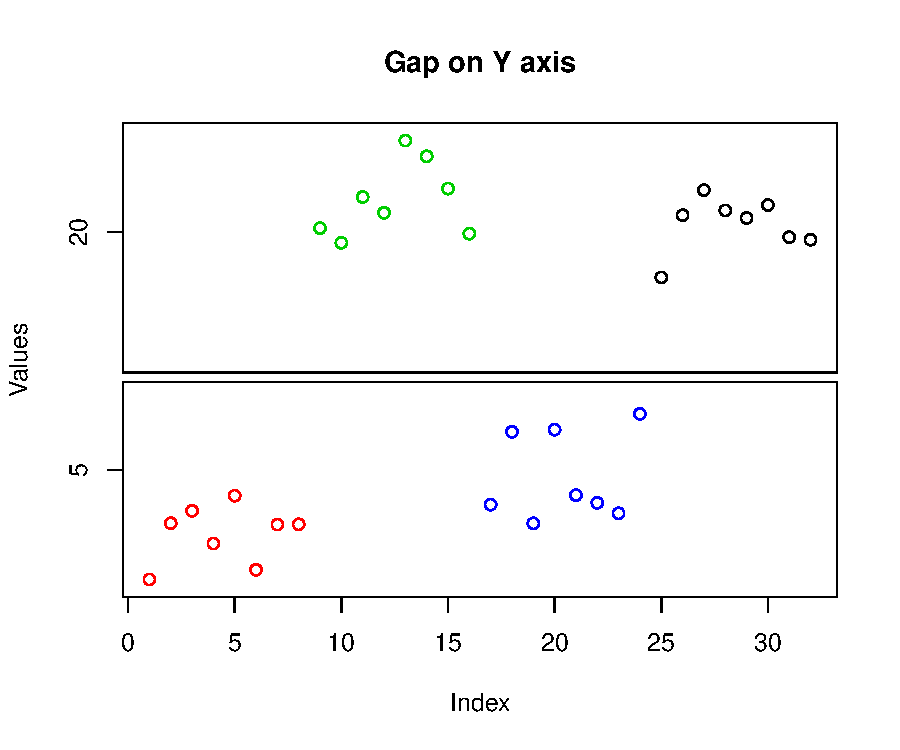
\includegraphics{plots/fig-026}
\end{frame}

\begin{frame}[fragile, allowframebreaks]
  \frametitle{Gap on a barplot}
  \begin{itemize}
  \item Or a barplot with a gap.
  \item Very helpful to visualize all your data.
  \item However, there is an issue with the labels on the $Y$ axis T\_T so be careful when using this kind of plot.
  \end{itemize}
\begin{Schunk}
\begin{Sinput}
> data <- c(rnorm(10), rnorm(10) + 
+     30)
> gap.barplot(data, gap = c(6, 25), 
+     xlab = "Index", ytics = c(1:30), 
+     ylab = "Group values", las = 2)
\end{Sinput}
\end{Schunk}
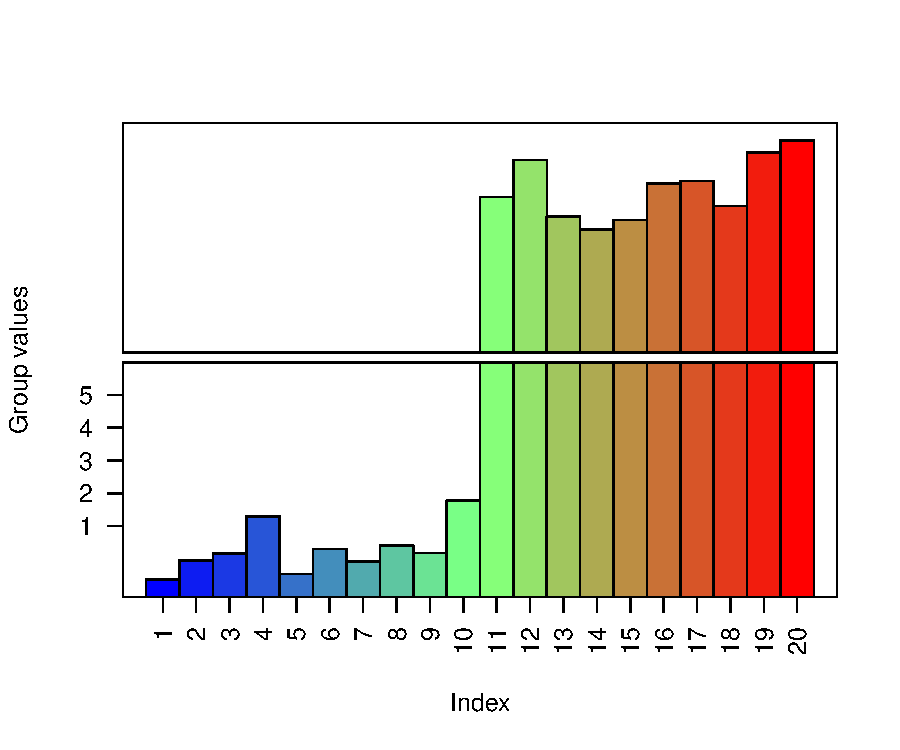
\includegraphics{plots/fig-027}
\end{frame}

\begin{frame}[fragile, allowframebreaks]
  \frametitle{Error bars}
  \begin{itemize}
  \item Nowadays you get to see lots of graphs with the error bars.
  \item Experimental papers generally have 3 to 5 repeats of the same experiment.
  \item The \BIOCfunction{dispersion} function will be helpful to make this kind of plot.
  \end{itemize}
\begin{Schunk}
\begin{Sinput}
> data <- matrix(rnorm(100), 10, 
+     10)
> a <- colMeans(data)
> b <- std.error(data)
> plot(a, ylim = c(min(a - b), max(a + 
+     b)), xlab = "Sample", ylab = "Value", 
+     col = 4, type = "o")
> dispersion(1:10, colMeans(data), 
+     b)
\end{Sinput}
\end{Schunk}
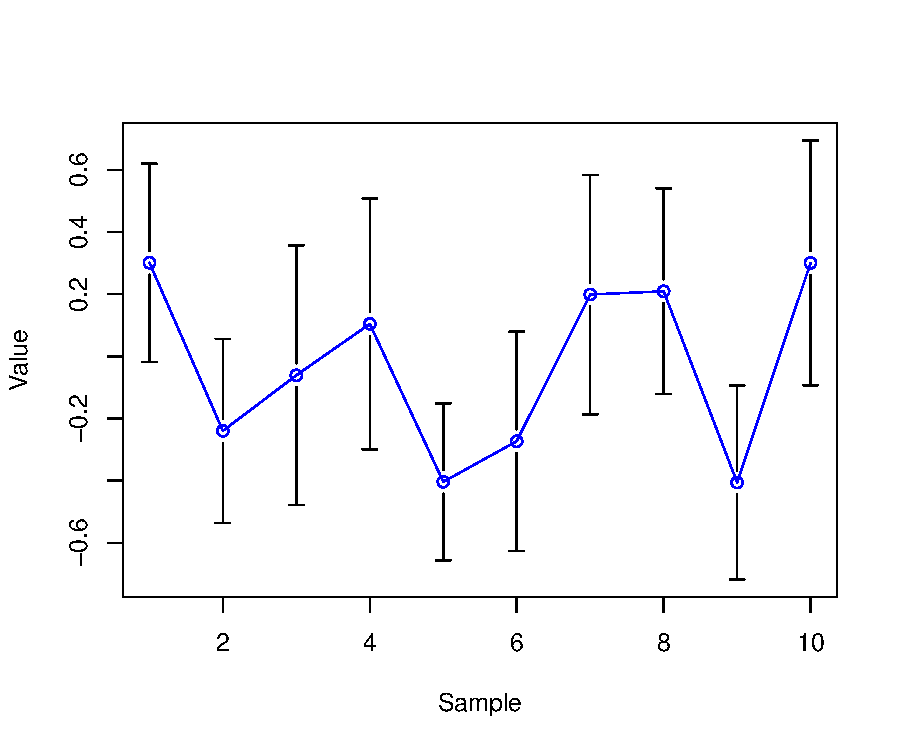
\includegraphics{plots/fig-028}
\end{frame}

\begin{frame}[allowframebreaks, fragile]
  \frametitle{Some real data}
  \begin{itemize}
  \item For the next plots, we'll use data from \myurlshort{www.ncbi.nlm.nih.gov/pubmed/19587683}{this article} where they sequenced a Korean individual.
  \item I already saved as \pl{csv} files two tables for easy import. We'll load them into \pl{R} with the \BIOCfunction{read.csv} function. \scriptsize
\begin{Schunk}
\begin{Sinput}
> t1 <- read.csv("http://www.lcg.unam.mx/~lcollado/B/data/SuppTable01_kogenome6_double_end-clone_1132_742.csv", 
+     header = T)
> t2 <- read.csv("http://www.lcg.unam.mx/~lcollado/B/data/SuppTable06_nsSnp_AK1.csv", 
+     header = T)
\end{Sinput}
\end{Schunk}
  \item \normalsize Use \alert{head}, \alert{dim}, \alert{class} to find out more about the data.
  \end{itemize}
\end{frame}

\begin{frame}[fragile, allowframebreaks]
  \frametitle{plotCI}
  \begin{itemize}
  \item \pl{Plotrix} has another function that plots error bars.
  \item We'll use our first table and get the data we need using \pl{tapply}.
  \end{itemize}
\begin{Schunk}
\begin{Sinput}
> means <- tapply(t1$bac_size, t1$chrNo, 
+     mean)
> err <- tapply(t1$bac_size, t1$chrNo, 
+     std.error)
> plotCI(1:24, means, err, col = "red", 
+     scol = "blue", las = 2, main = "bac_size per chrNo")
\end{Sinput}
\end{Schunk}
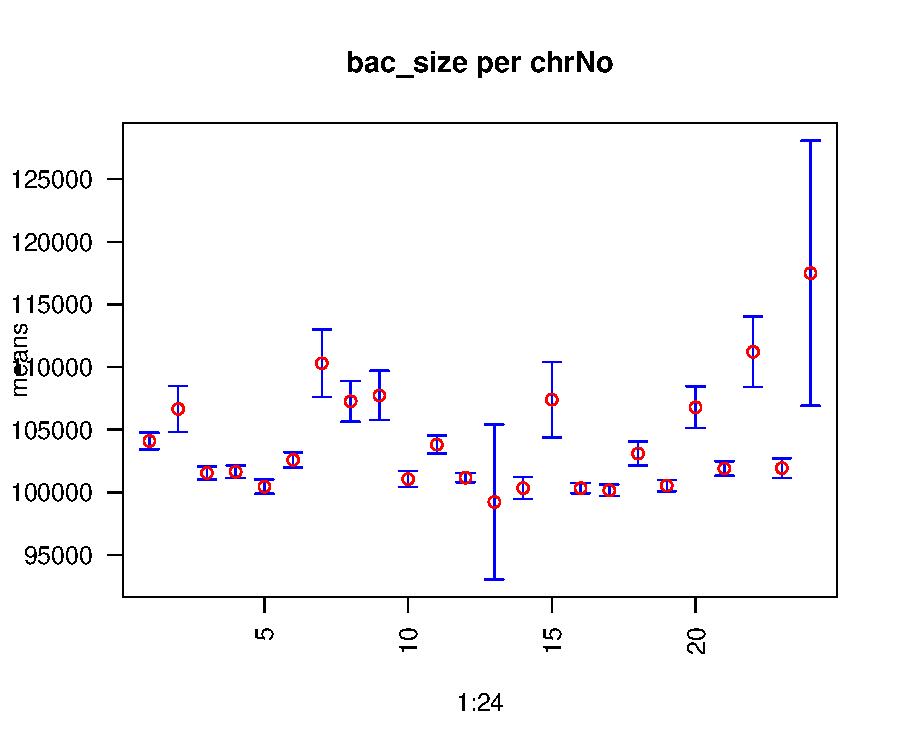
\includegraphics{plots/fig-030}
\end{frame}

\begin{frame}[fragile, allowframebreaks]
  \frametitle{One similar to image}
  \begin{itemize}
  \item With \BIOCfunction{color2D.matplot} we can make plots very similar to \pl{image}
  \item What differences do you notice vs \pl{image}?
  \end{itemize}
\begin{Schunk}
\begin{Sinput}
> mat <- matrix(rnorm(100, 0, 2), 
+     10, 10)
> color2D.matplot(mat, show.legend = T)
\end{Sinput}
\end{Schunk}
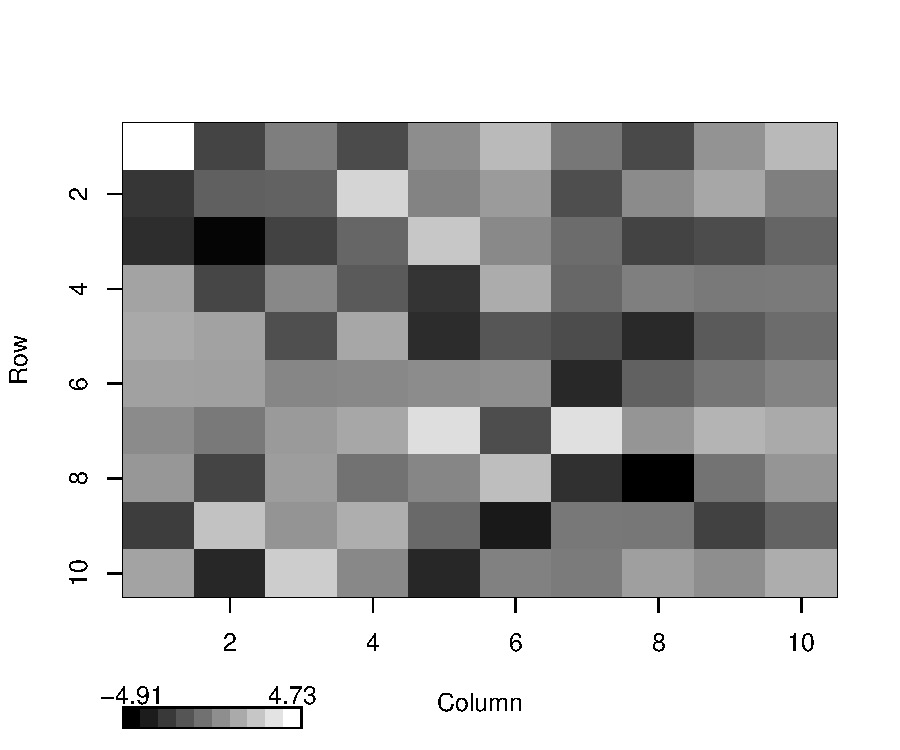
\includegraphics{plots/fig-031}
\end{frame}


\begin{frame}[fragile, allowframebreaks]
  \frametitle{Hierobarp}
  \begin{itemize}
  \item We'll use the default example for this powerful plot.
  \end{itemize}
\begin{Schunk}
\begin{Sinput}
> test.df <- data.frame(Age = rnorm(100, 
+     25, 10), Sex = sample(c("M", 
+     "F"), 100, TRUE), Marital = sample(c("D", 
+     "M", "S", "W"), 100, TRUE), 
+     Employ = sample(c("Full Time", 
+         "Part Time", "Unemployed"), 
+         100, TRUE))
> test.col <- list(Overall = "green", 
+     Employ = c("purple", "orange", 
+         "brown"), Marital = c("#1affd8", 
+         "#caeecc", "#f7b3cc", "#94ebff"), 
+     Sex = c(2, 4))
> hierobarp(formula = Age ~ Sex + 
+     Marital + Employ, data = test.df, 
+     ylab = "Mean age (years)", 
+     main = "Show only the final breakdown", 
+     errbars = TRUE, col = test.col$Sex)
\end{Sinput}
\end{Schunk}
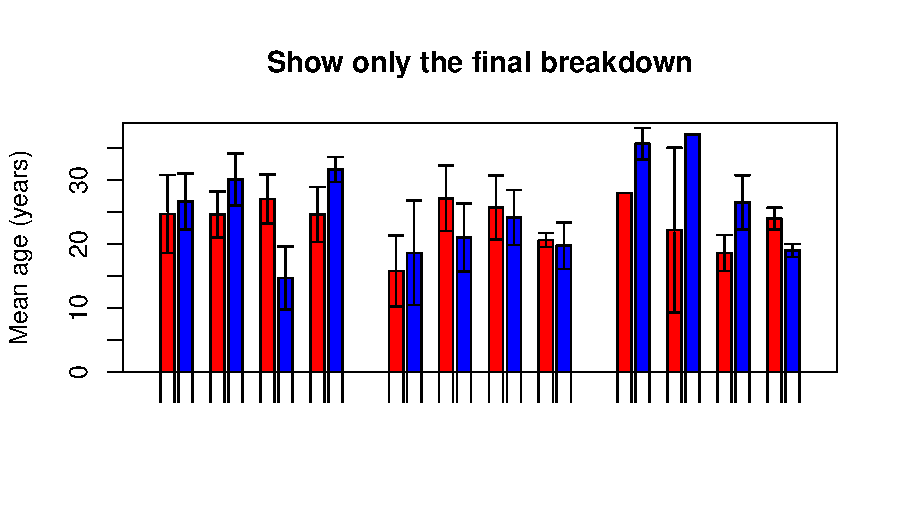
\includegraphics{plots/fig-032}
\end{frame}

\begin{frame}[fragile, allowframebreaks]
  \frametitle{Two scales}
  \begin{itemize}
  \item Sometimes you want two lines with different scales on the same plot.
  \item \BIOCfunction{twoord.plot} is the solution :)
  \end{itemize}
\begin{Schunk}
\begin{Sinput}
> twoord.plot(2:10, seq(3, 7, by = 0.5) + 
+     rnorm(9), 1:15, rev(60:74) + 
+     rnorm(15), xlab = "Sequence", 
+     ylab = "Ascending values", 
+     rylab = "Descending values", 
+     main = "Plot with two ordinates - points and lines")
\end{Sinput}
\end{Schunk}
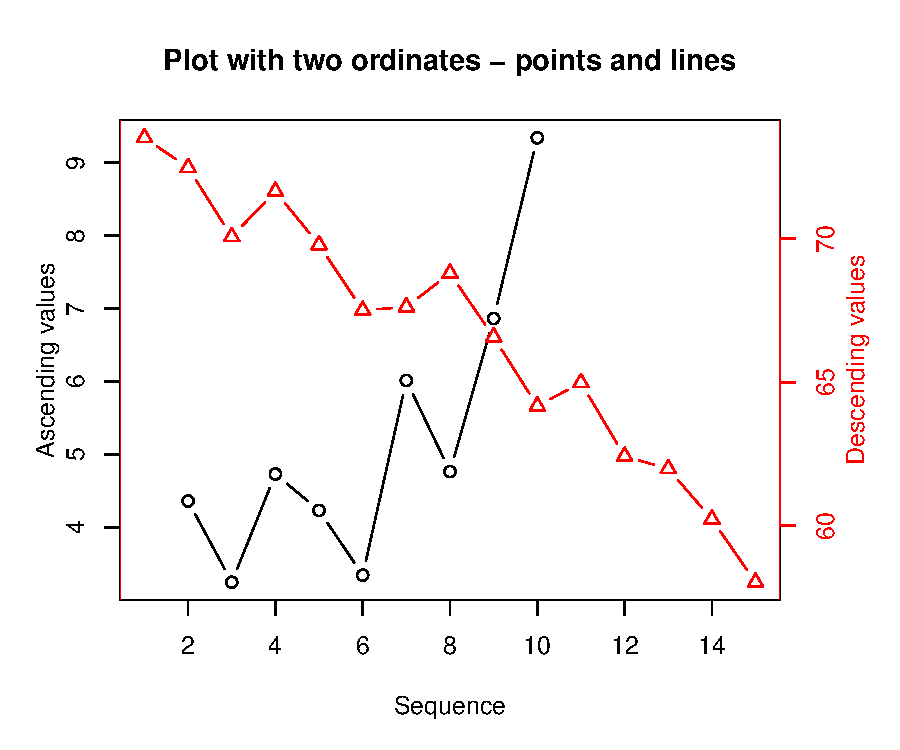
\includegraphics{plots/fig-033}
\end{frame}

\begin{frame}[fragile, allowframebreaks]
  \frametitle{Zoom}
  \begin{itemize}
  \item The final plot I'll show you from \pl{plotrix} enables us to zoom into a section of the plot.
  \end{itemize}
\begin{Schunk}
\begin{Sinput}
> zoomInPlot(rnorm(100), rnorm(100), 
+     rxlim = c(-1, 1), rylim = c(-1, 
+         1), zoomtitle = "Zoom In Plot")
\end{Sinput}
\end{Schunk}
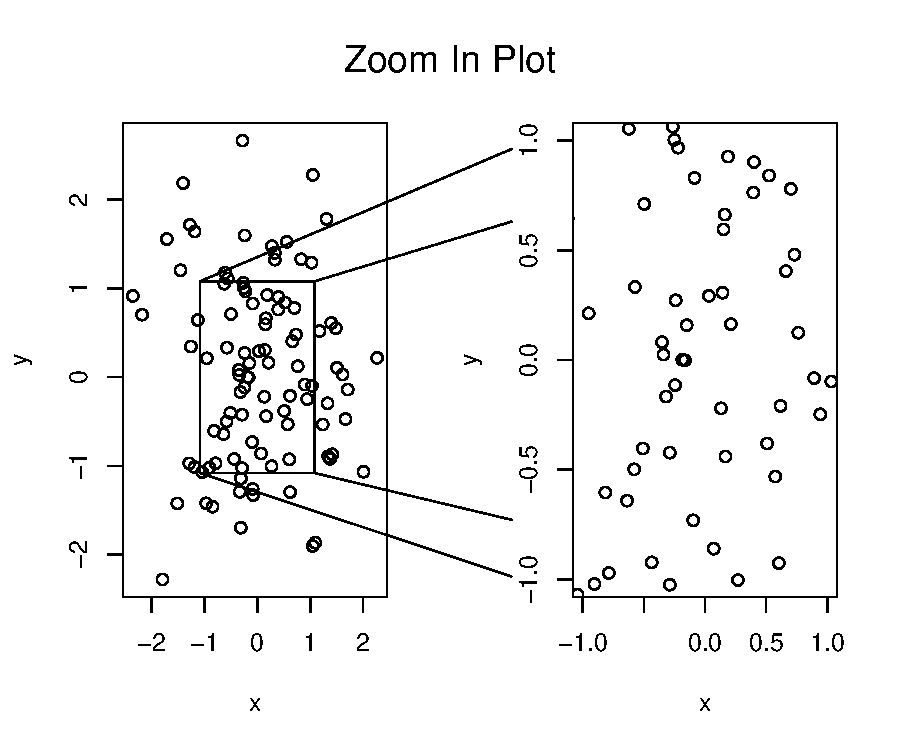
\includegraphics{plots/fig-034}
\end{frame}

%%%%%%%%%%%%%%%%%%%%%%%%%%%%%%%%%%%%%%%%%%%%%%%%%%%%%%%%%%%%%%%%%%%%%%%%%%%
\section{ggplot2}

\begin{frame}[allowframebreaks]
  \frametitle{Intro}
  \begin{itemize}
  \item \alert{ggplot2} is a much more sophisticated plotting package.
  \item \alert{199} pages long ref manual!!!
  \item Lets take a look at some examples.
  \end{itemize}
\end{frame}

\begin{frame}[fragile, allowframebreaks]
  \frametitle{Plotmatrix}
  \begin{itemize}
  \item We'll use the \BIOCfunction{iris} data set which is used quite frequently to exemplify scatterplots.
  \item Meaning that you are using 3 or more variables.
  \item Explore \pl{iris} with head and other similar functions.
  \end{itemize}
\begin{Schunk}
\begin{Sinput}
> plotmatrix(iris[, 1:4])
\end{Sinput}
\end{Schunk}
\end{frame}

\begin{frame}[fragile, allowframebreaks]
  \frametitle{Plotmatrix II}
  \begin{itemize}
  \item If we combine \BIOCfunction{plotmatrix} with \BIOCfunction{geom\_smooth} we can get a much better graph.
  \end{itemize}
\begin{Schunk}
\begin{Sinput}
> plotmatrix(iris[, 1:4]) + geom_smooth(method = "lm")
\end{Sinput}
\end{Schunk}
\end{frame}

\begin{frame}[fragile, allowframebreaks]
  \frametitle{We'll be back}
  \begin{itemize}
  \item On the class where we'll learn about linear regressions, we'll be back and make plots like this one:
  \end{itemize}
\begin{Schunk}
\begin{Sinput}
> mod <- lm(mpg ~ wt, data = mtcars)
> qplot(.fitted, .resid, data = mod) + 
+     geom_hline() + geom_smooth(se = FALSE)
\end{Sinput}
\end{Schunk}
\end{frame}

%%%%%%%%%%%%%%%%%%%%%%%%%%%%%%%%%%%%%%%%%%%%%%%%%%%%%%%%%%%%%%%%%%%%%%%%%%%
\section{car}

\begin{frame}[allowframebreaks]
  \frametitle{Intro}
  \begin{itemize}
  \item While this package has quite a lot of functions too (105 page ref man), one special plot caught my eye.
  \item Feel free to check all the examples later if you want :D
  \end{itemize}
\end{frame}

\begin{frame}[fragile, allowframebreaks]
  \frametitle{scatterplot.matrix}
  \begin{itemize}
  \item Quite similar plot to some we made before with automatic colors
  \end{itemize}
\begin{Schunk}
\begin{Sinput}
> library(car)
> scatterplot.matrix(~income + education + 
+     prestige | type, data = Duncan)
\end{Sinput}
\end{Schunk}
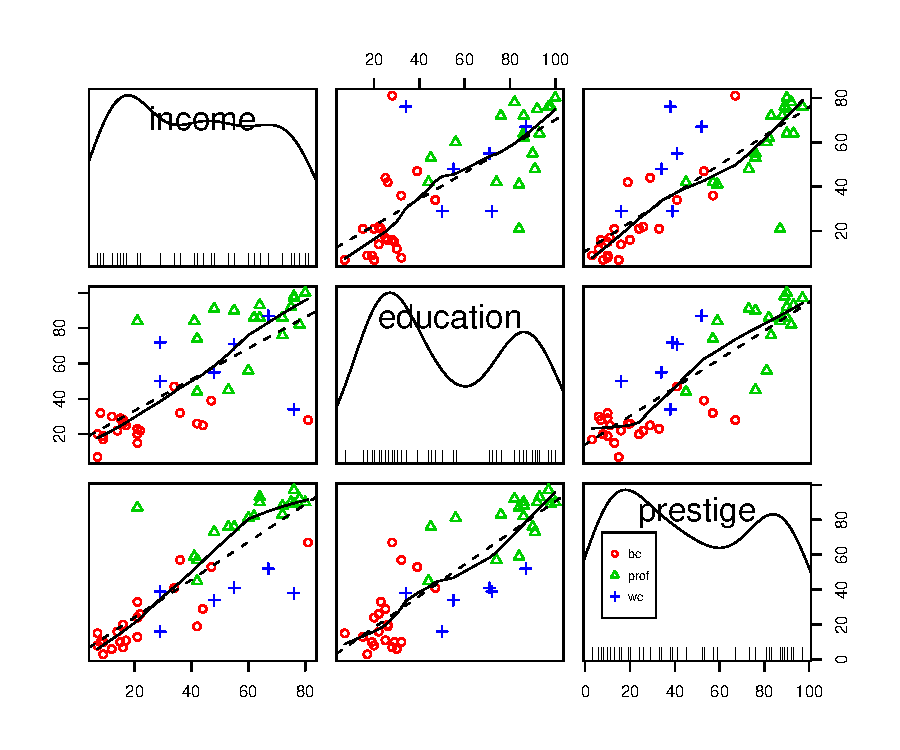
\includegraphics{plots/fig-038}
\end{frame}

\begin{frame}[fragile, allowframebreaks]
  \frametitle{scatterplot}
  \begin{itemize}
  \item With \BIOCfunction{scatterplot} we can create boxplots on our axis!!
  \end{itemize}
\begin{Schunk}
\begin{Sinput}
> scatterplot(prestige ~ income | 
+     type, data = Prestige, span = 1)
\end{Sinput}
\end{Schunk}
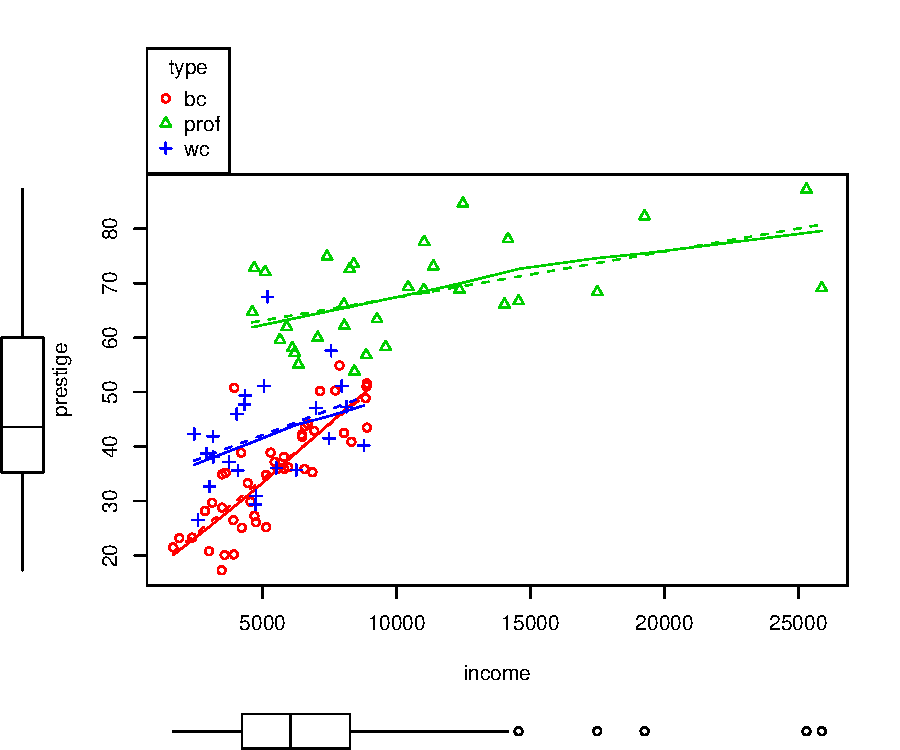
\includegraphics{plots/fig-039}
\end{frame}

\begin{frame}[allowframebreaks, fragile]
  \frametitle{Session Info}
  \scriptsize
\begin{Schunk}
\begin{Sinput}
> sessionInfo()
\end{Sinput}
\begin{Soutput}
R version 2.10.0 Under development (unstable) (2009-07-21 r48968) 
i386-pc-mingw32 

locale:
[1] LC_COLLATE=English_United States.1252 
[2] LC_CTYPE=English_United States.1252   
[3] LC_MONETARY=English_United States.1252
[4] LC_NUMERIC=C                          
[5] LC_TIME=English_United States.1252    

attached base packages:
[1] stats     graphics  grDevices
[4] utils     datasets  methods  
[7] base     

other attached packages:
[1] car_1.2-15         
[2] plotrix_2.6-4      
[3] DAAG_1.00          
[4] randomForest_4.5-30
[5] rpart_3.1-44       
[6] MASS_7.3-0         
[7] lattice_0.17-25    

loaded via a namespace (and not attached):
[1] grid_2.10.0  tools_2.10.0
\end{Soutput}
\end{Schunk}
\end{frame}

\end{document}
